\section{Cahier des charges}

Nous avons eu l'occasion d'échanger avec les membres de Kerpape, ce qui nous a permis de définir le cahier des charges de l'application, que nous allons détailler dans cette partie.

\subsection{Partie fonctionnelle}

En effet, l'utilisation des appartements tremplins qui permet la mise en situation des patients dans un environnement réel, rencontre des difficultés avec les patients ayant des troubles cognitifs. La domotique trés présente dans l'appartement rencontre donc des difficultés de compréhension et d'utilisation de la part des patients, d'où l'idée d'un environement virtuel d'apprentissage en amont.

\subsubsection{Modes de fonctionnement}

Le programme doit comporter trois modes d'utilisation dont deux assistent en partie l'utilisateur pour son apprentissage. Le troisième permet une interaction avec l'environnement de manière plus autonome.\\

\textbf{Apprentissage symbolique}
\\

Ce mode doit permettre de tout apprendre depuis le début et de comprendre le fonctionnement global des différentes situations auxquelles l'utilisateur peut être confronté. Il comporte des vues statiques, \enquote{zoomées}, avec la mise en évidence d'actions à réaliser, ainsi que des indications visuelles symboliques.\\

\textbf{Assisté}
\\

Dans un environnement réaliste, le logiciel donne des indications légères pour permettre de retrouver les actions à faire. Ces indications sont activables par les ergothérapeutes. Par exemple :
\begin{itemize}
  \item la surbrillance des objets à actionner,
  \item lors de l'activation d'une action on accède à une vue fixe avec les états courants des équipements afin de faciliter la compréhension du lien action/objet pour l'utilisateur. \\
\end{itemize}

\textbf{Autonome}
\\

L'utilisateur ne reçoit plus d'information ou d'indication pour effectuer son parcours, il est dans le décor le plus réaliste possible, pour valider son autonomie. Il doit alors actionner les différents objets et se rendre compte par lui même (déplacement) des actions qu'il a effectuées.

\subsubsection{Points de vue : exocentré, endocentré}

Deux points de vue sont configurables. Une vue à la troisième personne (exocentrée) permet de voir le déplacement de l'utilisateur dans la scène.
Grâce à cette vue, l'utilisateur peut mieux voir les interactions avec son environnement et avoir une vision plus globale sur la scène. 
On peut ainsi avoir des angles de caméra qu'un avatar virtuel ne pourrait avoir ; il est par exemple possible de voir à la fois devant et derrière soi (cf.\textsc{figure~\ref{exo}}).
\newline
Une vue à la première personne (endocentrée) sera aussi incluse, permettant une immersion totale dans la scène. 
En effet, ce type de vision est proche du point de vue humain, ce qui permet une identification facile à l'avatar virtuel pour l'utilisateur. C'est donc le type de vue le plus logique en réalité virtuelle (cf. \textsc{figure~\ref{endo}}).
%\noindent
\begin{figure}[h]
	\begin{minipage}[b]{0.3\textwidth}
		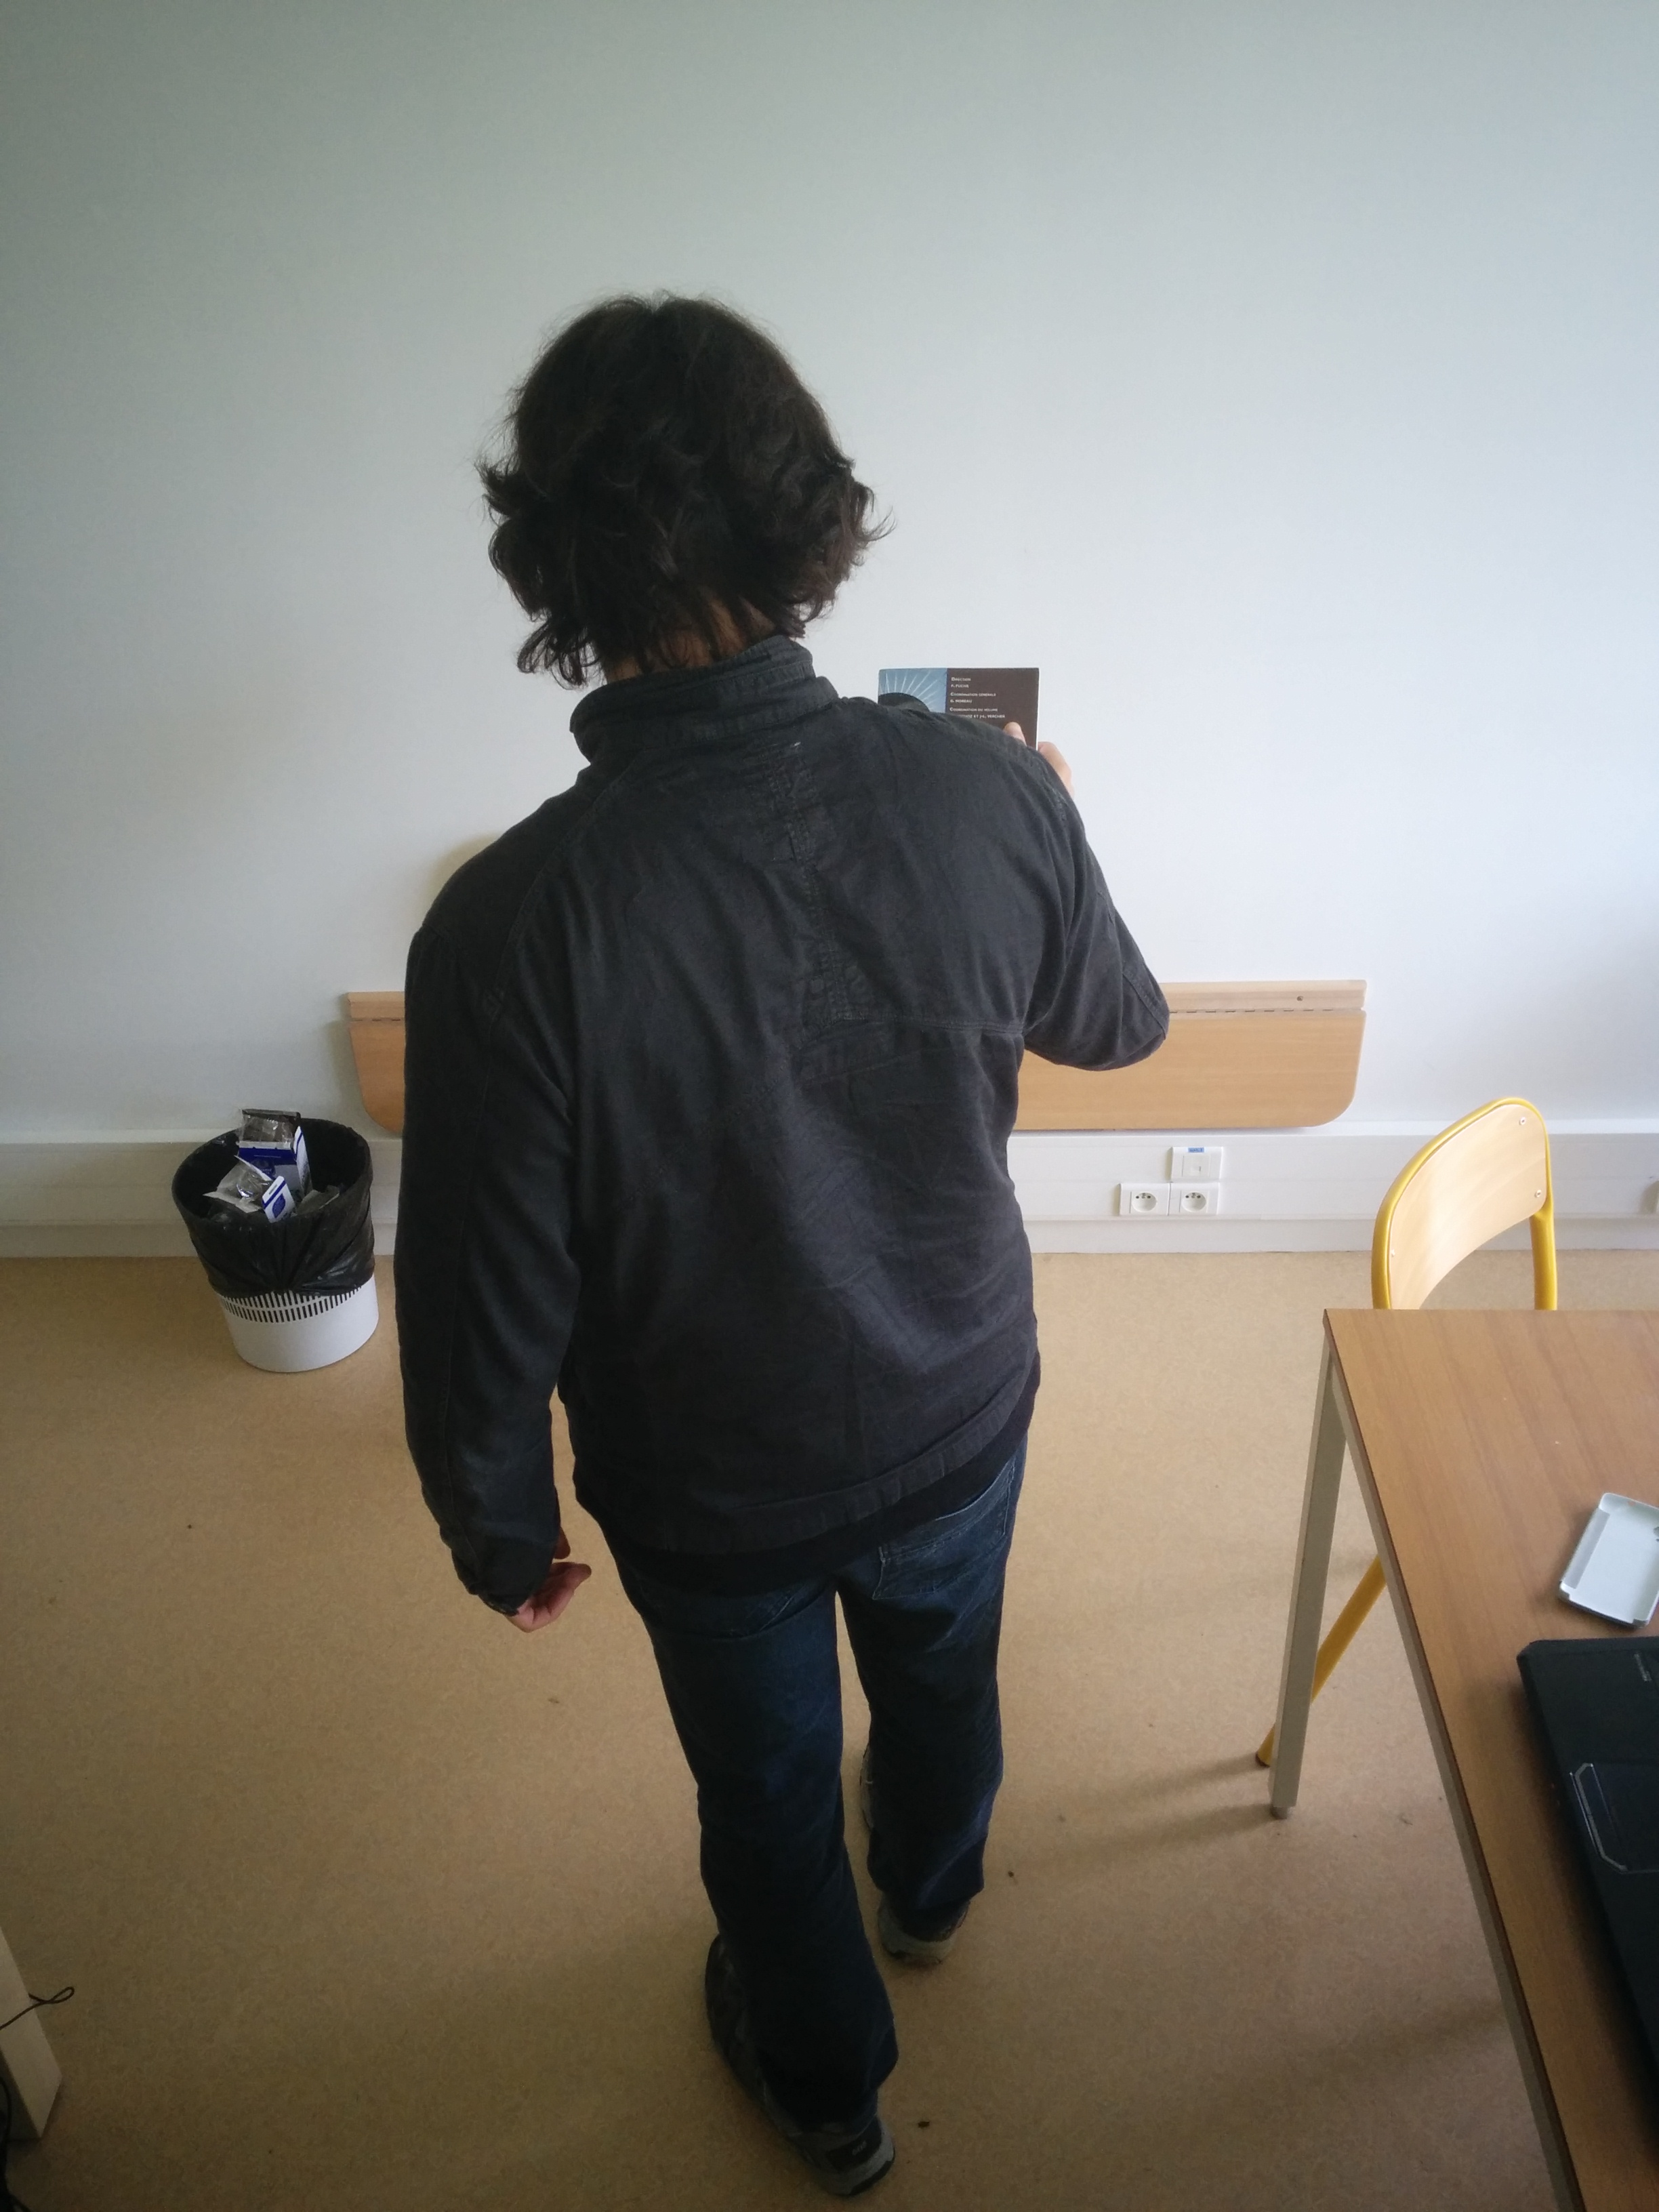
\includegraphics[width=\linewidth]{1-PreEtude/img/vue_tps}
		\caption{Vue exocentrée}
		\label{exo}
	\end{minipage}
	\begin{minipage}[b]{0.3\textwidth}
		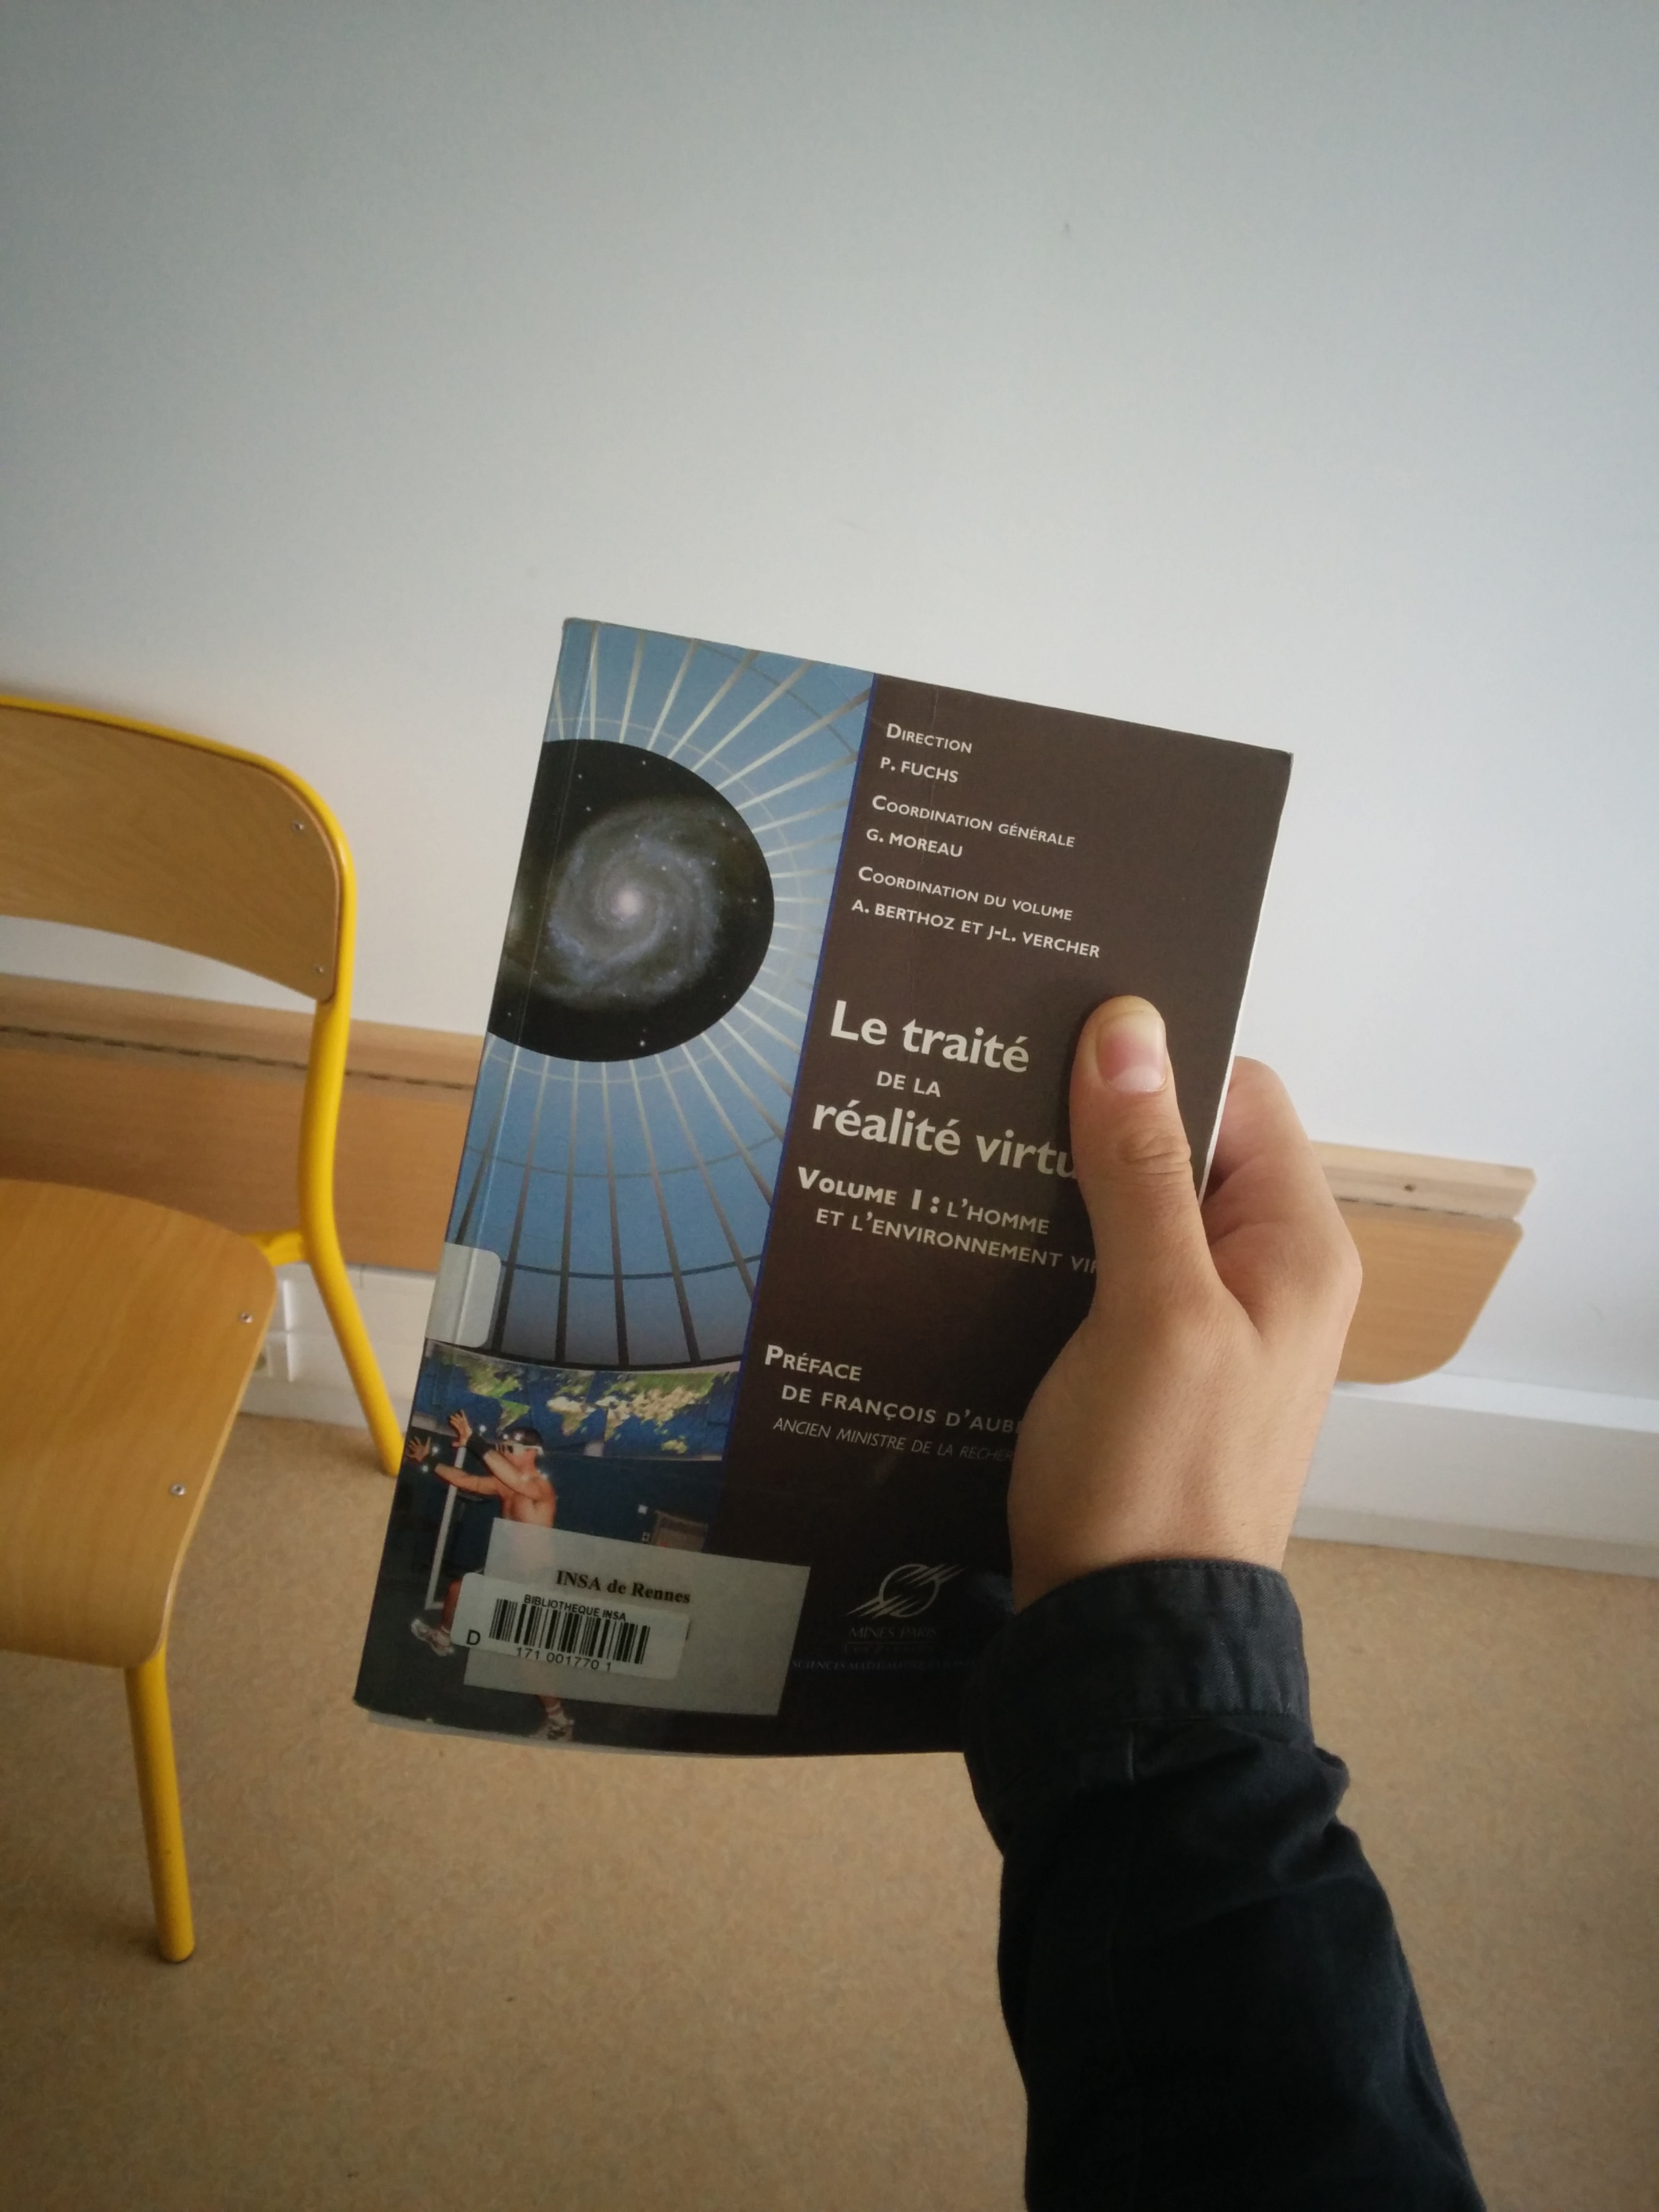
\includegraphics[width=\linewidth]{1-PreEtude/img/vue_fps}
		\caption{Vue endocentrée}
		\label{endo}
	\end{minipage}
%		\hfill
\end{figure}
\subsubsection{Déplacements, mise en situation et interactions}

L'utilisateur peut se déplacer librement dans l'appartement en mode autonome ; en parallèle il peut choisir de se mettre en situation sur les différents scénarios proposés afin d'interagir avec les différents objets prévus pour le scénario.

Centrées autour d'un bloc d'interrupteurs, les interactions comprennent notamment pouvoir ouvrir ou fermer les portes (porte du hall avec fermeture automatique, de l'appartement avec fermeture volontaire), d'allumer ou éteindre les lumières (commande variateur, commande interrupteur) et de monter ou descendre les volets.

\subsubsection{Scénarios}
Trois scénarios autour de l'appel sur le téléphone sont à prévoir avec des actions différentes à entreprendre décrites dans l'étude fonctionnelle. \\

\textbf{Appel téléphonique: }\textit{Appel téléphonique (d'un proche ou d'une personne qui se serait trompée de numéro). }
%- L'utilisateur doit pouvoir décrocher le téléphone pour entrer en communication puis raccrocher quand la communication est terminée.

\textbf{Interphone infirmier: } \textit{Appel venant du portier audio/vidéo sur le téléphone (d'un infirmier qui souhaiterait entrer). }
%L'utilisateur doit pouvoir décrocher le téléphone, communiquer avec l'infirmier, raccrocher le téléphone et ouvrir la porte.

\textbf{Interphone inconnu: } \textit{Appel venant du portier audio/vidéo sur le téléphone (d'un inconnu). }
%L'utilisateur doit pouvoir décrocher le téléphone pour entrer en communication, allumer la TV pour voir la vidéo puis éteindre la TV et raccrocher le téléphone à la fin de la conversation.

\subsection{Partie technique}

Notre application va présenter un certain nombre d'axes de développement à respecter, que nous allons définir ici : la présence d'interactions avec l'environnement, faire une application aisément portable sur différents systèmes d'utilisation, et enfin une application capable de fonctionner avec de nombreux périphériques différents. 

\subsubsection{Interactions et 3D en temps réel}
L'utilisateur doit pouvoir interagir avec son environnement. Il ne s'agit pas d'un film ou d'un logiciel présentant un scénario fixe ; l'environnement doit évoluer en fonction des actions de l'utilisateur.

Pour représenter notre environnement virtuel, nous allons devoir générer des images d'une modélisation 3D de l'appartement. Ces images ne sont pas figées et évoluent avec la position de l'utilisateur ou la modification de son environnement. Il s'agit donc de générer un flux continu d'images pour avoir un rendu fluide, à l'aide d'un moteur de rendu 3D en temps réel. La scène doit être suffisement simple pour que l'on puisse obtenir une moyenne suffisante d'images par seconde.

\subsubsection{Plate-forme d'exécution}

Dans un premier temps, nous ciblons un ordinateur fonctionnant sous Windows 7/8 à l'aide d'un clavier et d'une souris. Cependant, il serait dommage d'être coincé dans cet environnement par nos choix de bibliothèques et programmes tiers. Nous allons donc chercher à utiliser un moteur 3D proposant plusieurs cibles de compilation et ne nous limitant pas sur le choix des périphériques, pour pouvoir éventuellement porter le logiciel sur tablette ou le faire tourner sur une plate-forme telle qu'une salle immersive ou bien un casque de réalité virtuelle.

\subsubsection{Abstraction des périphériques}

Nous devons réfléchir aux différents environnements dans lesquels notre logiciel pourra évoluer : il s'agira d'abord de le faire fonctionner sur une plate-forme très commune composée d'un écran et d'un clavier ; mais nous devons également réfléchir à la future intégration d'autres périphériques. Pour se rapprocher de la réalité, nous pourrions utiliser de réels interrupteurs associés à des capteurs de position comme périphériques d'entrée. L'image pourrait quant à elle être diffusée sur un périphérique de réalité virtuelle comme un casque de réalité virtuelle.

Afin de ne pas devoir réécrire l'ensemble de la couche entrées/sorties de notre logiciel, il est intéressant de se tourner vers une solution d'abstraction matérielle permettant d'ajouter des périphériques simplement.
